\documentclass[tikz,border=3mm]{standalone}
\usetikzlibrary{arrows.meta, positioning}

\begin{document}
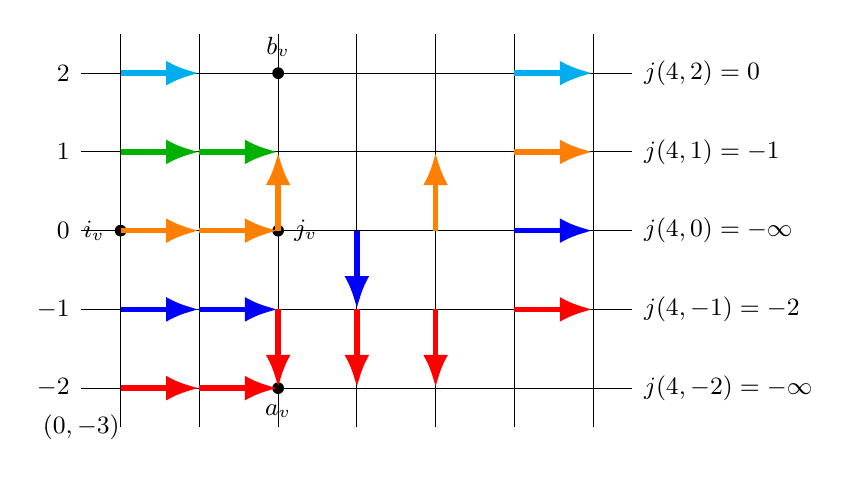
\begin{tikzpicture}[scale=1.0, 
    >=Latex,
    font=\small,
    myarrow/.style={->, line width=2pt, color=#1},
    dot/.style={circle, fill, inner sep=1.5pt},
    every label/.append style={font=\small}
]

% Left side diagram
\node[dot, label={left:$i_v$}] (i) at (-2,0) {};
\node[dot, label={right:$j_v$}] (j) at (0,0) {};
\node[dot, label={below:$a_v$}] (a) at (0,-2) {};
\node[dot, label={above:$b_v$}] (b) at (0,2) {};

\draw (i) -- (j);
\draw (j) -- (a);
\draw (j) -- (b);

% Right side grid
\foreach \x in {-2,...,4} {
    \draw (\x,-2.5) -- (\x,2.5);
}
\foreach \y in {-2,...,2} {
    \draw (-2.5,\y) -- (4.5,\y);
}

% Drawing arrows and labeling
\draw[myarrow=cyan] (-2,2) -- (-1,2);
\draw[myarrow=green!70!black] (-2,1) -- (-1,1);
\draw[myarrow=orange] (-2,0) -- (-1,0);
\draw[myarrow=blue] (-2,-1) -- (-1,-1);
\draw[myarrow=red] (-2,-2) -- (-1,-2);

\node[label={[label distance=-1mm]left:$2$}] at (-2.5,2) {};
\node[label={[label distance=-1mm]left:$1$}] at (-2.5,1) {};
\node[label={[label distance=-1mm]left:$0$}] at (-2.5,0) {};
\node[label={[label distance=-1mm]left:$-1$}] at (-2.5,-1) {};
\node[label={[label distance=-1mm]left:$-2$}] at (-2.5,-2) {};

% Colorful arrows within the grid
\draw[myarrow=green!70!black] (-1,1) -- (0,1);
\draw[myarrow=orange] (-1,0) -- (0,0);
\draw[myarrow=blue] (-1,-1) -- (0,-1);
\draw[myarrow=red] (-1,-2) -- (0,-2);

\draw[myarrow=orange] (0,0) -- (0,1);
\draw[myarrow=red] (0,-1) -- (0,-2);

\draw[myarrow=blue] (1,0) -- (1,-1);
\draw[myarrow=red] (1,-1) -- (1,-2);

\draw[myarrow=orange] (2,0) -- (2,1);
\draw[myarrow=red] (2,-1) -- (2,-2);

\draw[myarrow=cyan] (3,2) -- (4,2);
\draw[myarrow=orange] (3,1) -- (4,1);
\draw[myarrow=blue] (3,0) -- (4,0);
\draw[myarrow=red] (3,-1) -- (4,-1);

\node[label={[label distance=-1mm]right:$j(4,2)=0$}] at (4.5,2) {};
\node[label={[label distance=-1mm]right:$j(4,1)=-1$}] at (4.5,1) {};
\node[label={[label distance=-1mm]right:$j(4,0)=-\infty$}] at (4.5,0) {};
\node[label={[label distance=-1mm]right:$j(4,-1)=-2$}] at (4.5,-1) {};
\node[label={[label distance=-1mm]right:$j(4,-2)=-\infty$}] at (4.5,-2) {};

% Label for the bottom-left corner
\node at (-2.5,-2.5) {$(0,-3)$};

\end{tikzpicture}
\end{document}